\documentclass{report}
\usepackage{amsmath}
\usepackage{graphicx}
\usepackage{booktabs}

\title{Labwork 4: 2D Threads Configuration}
\author{Nguyen Duy Anh Tung}
\date{\today}

\begin{document}
\maketitle

\section{Introduction}
In Labwork 4, we extend the RGB-to-grayscale conversion by comparing a 1D flattened grid layout with a 2-dimensional thread and block hierarchy. The objective is to preserve the native 2D spatial representation of images, benchmark performance across various block geometries, evaluate hardware constraints, and solve classroom exercises on thread occupancy.

\section{Implementation}
We benchmark two parallel CUDA approaches against a sequential CPU baseline:
\begin{itemize}
    \item \textbf{Sequential CPU}: Processes the image matrix sequentially through nested height ($y$) and width ($x$) loops using the average formula $g = \lfloor(R + G + B) / 3\rfloor$.
    \item \textbf{1D CUDA Kernel}: Uses a flattened array of size $(N, 3)$, with thread indexing $tidx = \text{threadIdx.x} + \text{blockIdx.x} \times \text{blockDim.x}$.
    \item \textbf{2D CUDA Kernel}: Maintains the native $(H, W, 3)$ shape and computes 2D coordinates:
    \[
    x = \text{threadIdx.x} + \text{blockIdx.x} \times \text{blockDim.x}
    \]
    \[
    y = \text{threadIdx.y} + \text{blockIdx.y} \times \text{blockDim.y}
    \]
    A boundary check \texttt{if x < w and y < h} avoids out-of-bounds accesses.
\end{itemize}

\section{Experimental Results}
Testing was conducted on an image with $199,875$ pixels ($H \times W$). The sequential CPU execution time was \textbf{0.1967 s} ($196.7\text{ ms}$). GPU execution times are averaged over $5$ iterations.

\begin{table}[htbp]
\centering
\begin{tabular}{lrrrr}
\toprule
\textbf{Configuration} & \textbf{Threads/Block} & \textbf{Grid Size} & \textbf{GPU Time (ms)} & \textbf{Speedup} \\
\midrule
\multicolumn{5}{l}{\textit{1D Grid Hierarchy}} \\
32   & 32   & 6247 & 0.14 & $1449.8\times$ \\
64   & 64   & 3124 & 0.12 & $1665.1\times$ \\
128  & 128  & 1562 & 0.12 & $1636.7\times$ \\
256  & 256  & 781  & 0.12 & $1662.5\times$ \\
512  & 512  & 391  & 0.12 & $\mathbf{1680.8\times}$ \\
1024 & 1024 & 196  & 0.12 & $1587.6\times$ \\
\midrule
\multicolumn{5}{l}{\textit{2D Grid Hierarchy}} \\
$(4, 4)$   & 16   & $(94, 134)$ & 0.19 & $1016.4\times$ \\
$(8, 8)$   & 64   & $(47, 67)$  & 0.13 & $1557.6\times$ \\
$(16, 16)$ & 256  & $(24, 34)$  & 0.13 & $1517.5\times$ \\
$(32, 16)$ & 512  & $(12, 34)$  & 0.12 & $\mathbf{1585.2\times}$ \\
$(32, 32)$ & 1024 & $(12, 17)$  & 0.13 & $1503.1\times$ \\
\bottomrule
\end{tabular}
\caption{Performance comparison between 1D and 2D CUDA configurations}
\end{table}

\begin{figure}[htbp]
\centering
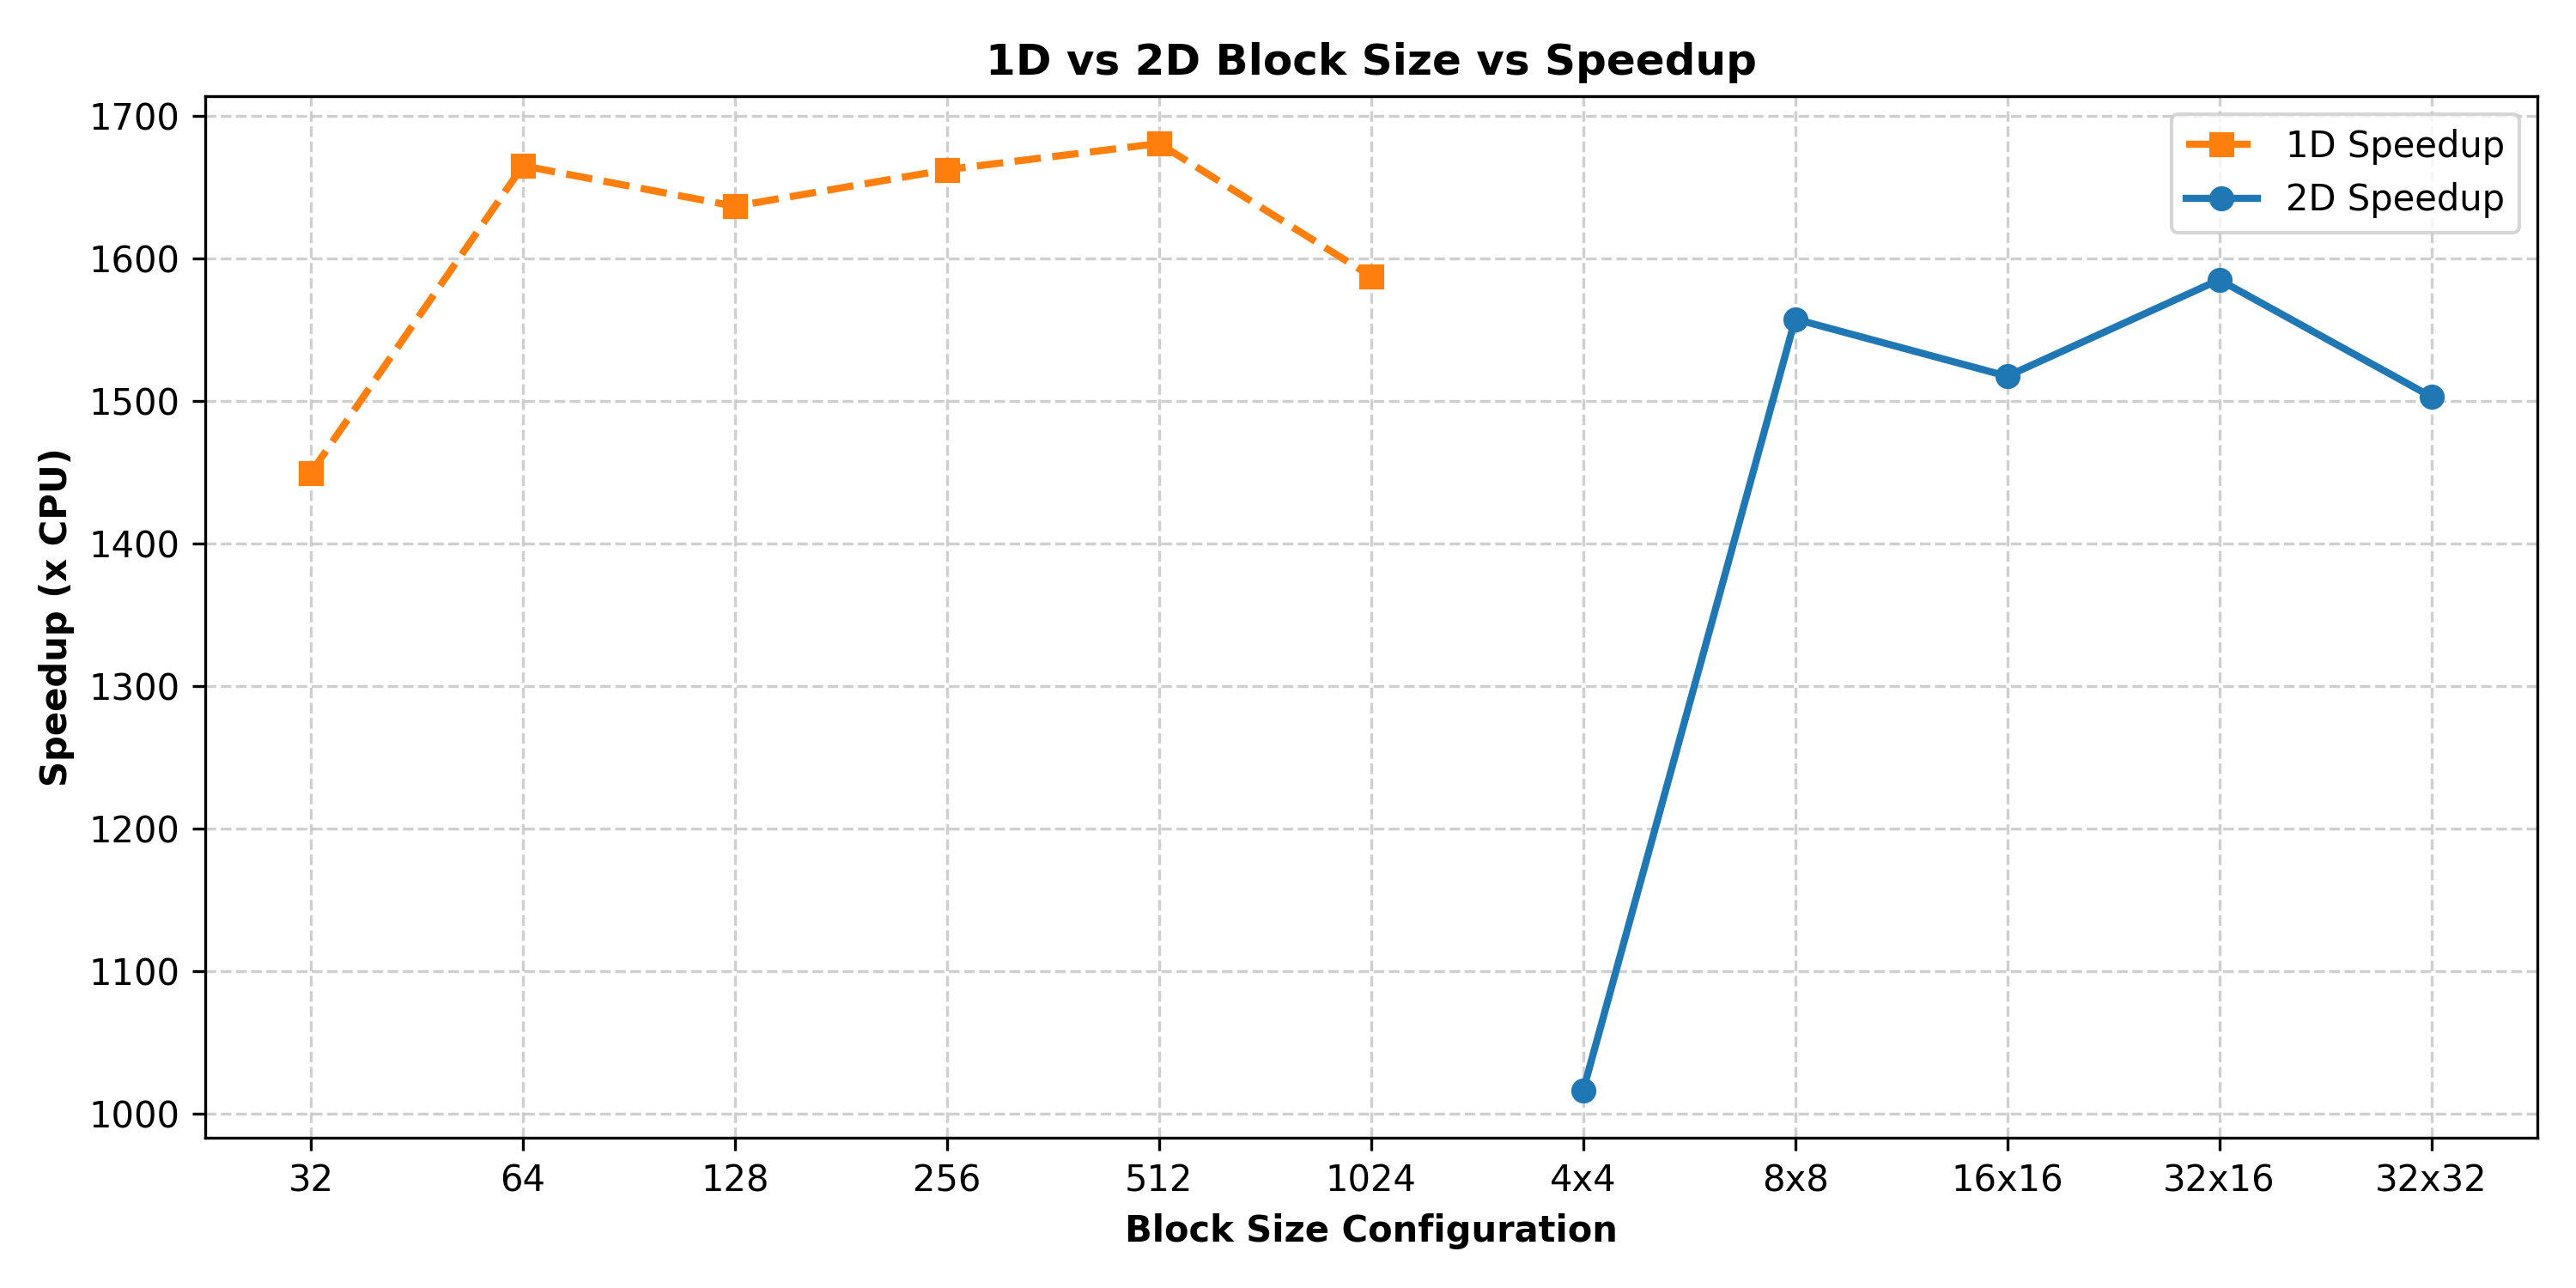
\includegraphics[width=0.85\textwidth]{block_size_vs_speedup.png}
\caption{1D vs 2D Block Size vs Speedup over CPU}
\end{figure}

\section{Hardware Limit and Crash Analysis}
When attempting configurations such as $(64, 32)$ ($2048$ threads) or $(64, 64)$ ($4096$ threads) for 2D version and threads bigger than 1024 for 1D version, the kernel execution crashes with:
\[
\texttt{numba.cuda.cudadrv.driver.CudaAPIError: [1] CUDA\_ERROR\_INVALID\_VALUE}
\]
This occurs because the NVIDIA CUDA architecture strictly limits the maximum number of threads in a single block to \textbf{1024} (\texttt{MAX\_THREADS\_PER\_BLOCK = 1024}). Configuration $(32, 32) = 1024$ represents the maximum allowable limit.

\section{Discussion}
\begin{itemize}
    \item \textbf{1D vs 2D Comparison}: Both layouts achieve comparable execution times ($\approx 0.12 - 0.13\text{ ms}$). The 1D layout slightly leads at peak speedup ($1680.8\times$ vs $1585.2\times$) due to flat linear indexing and continuous memory coalescing. However, 2D blocks provide natural geometric alignment for 2D spatial filtering.
    \item \textbf{Warp Sizing}: The $(4, 4)$ block ($16$ threads) performs worse ($0.19\text{ ms}$, $1016.4\times$) because it is smaller than the hardware warp size ($32$ threads), causing half the warp execution lanes to remain idle.
    \item \textbf{Optimal 2D Range}: Peak 2D performance occurs at $(32, 16)$ ($512$ threads, $0.12\text{ ms}$, $1585.2\times$), maintaining full warp occupancy and maximizing SM throughput.
    \item \textbf{Square vs. Non-Square Blocks}: The non-square configuration $(32, 16)$ achieves the best 2D performance ($0.12\text{ ms}$, $1585.2\times$). In CUDA, threads along the x-dimension form consecutive memory addresses in row-major order. By setting $\text{blockDim.x} = 32$ (exactly one full warp), all 32 threads in each warp access continuous horizontal pixels in global memory simultaneously, maximizing memory coalescing. In contrast, smaller x-dimensions (such as $(8, 8)$ and $(16, 16)$) require warps to span across multiple rows or require additional block scheduling, making $(32, 16)$ slightly more hardware-friendly than symmetric square blocks.
\end{itemize}

\end{document}